\chapter{Background}

%<Paragraph> Overview of background

This chapter provides a background on molecular computation techniques.  We begin with an introduction to nanotechnology and then provide an example of encoding information with molecular matter.  Following this example, we introduce Adleman's molecular operators for solving an instance of {\sc Hamiltonian Path}.  The operators provide a base instruction set for molecular computing, and provide the primitives to construct molecular algorithms.

In the second half of this chapter, we provide an introduction to {\sc Satisfiability}.  We define {\sc Satisfiability} as a circuit.  We then view {\sc Satisfiability} as a language.  We also discuss practical matters related to efficiently evaluating {\sc Satisfiability}, such as how to encode input and output, and how to classify instances of {\sc Satisfiability} for the test cases that we consider.

\section{On nanotechnology and construction of molecules}

%		<Paragraph> Richard Feynman [introduces] nanotechnology
		
	Richard Feynman founded the field of nanotechnology in his 1959 talk `There's Plenty of Room at the Bottom' \cite{feynman1959}.  Examples of applied nanotechnology include the manufacturing of graphene \cite{Stankovich_Dikin_Dommett_Kohlhaas_Zimney_Stach_Piner_Nguyen_Ruoff_2006} and DNA nanopores \cite{dnaTransistorIBMpressrelease}. Graphene consists of a planer arrangement of carbon atoms that provides desirable physical and electrical properties \cite{Stankovich_Dikin_Dommett_Kohlhaas_Zimney_Stach_Piner_Nguyen_Ruoff_2006}. DNA nanopores create a physical channel reading genetic sequences \cite{Garaj2010}.  Gene sequencing technologies provide an example of applied nanotechnology \cite{Garaj2010, ionTorrent, oxfordNanopore}.  					
			%The work has driven the fields of molecular and quantum computation, VLSI circuit construction, and continues with innovative design and applications into many everyday processes.
		
%		<Paragraph> DNA substrate [builds] molecular definition
		
Smaller and cost-effective DNA sequencers provide the ability to read the contents of a gene.  Benchtop sequencers \cite{ionTorrent, oxfordNanopore} allows doctors to treat patients at the genome level from their office.  Life Technologies and Oxford Nanopore offer gene sequencers based on solid-state semiconductor technology \cite{ionTorrent, oxfordNanopore}.	

\section{On microbiology and computation}

%	<Paragraph> Microbiology [studies] molecular life
	
	Microbiology studies the interactions among organic molecules.  In this project, we explore techniques from applied genetics as a means for generalized computation.  Molecular computation encodes data as sequences of DNA or RNA.  
	
%	<Paragraph> Genetic alphabet [defines] life
		
%	The genetic alphabet defines a universal medium for proteins.  Each of the nucleotides (A, C, G, T, U) transcribes redundant encodings of amino acids.  Sequences of amino acids form structure as proteins.  Redundant encodings in the each amino acid permit syntax errors without a functional abnormality.  This redundant encoding structure permits mutation in the third nucleotide of each amino acid without consequence on the entire string.

%	<Paragraph> Complex molecules [contain] unique strings 
	
	Strings of nucleotides encode information as oligonucleotides.  A \textit{oligonucleotide} is a short string of genetic information.  There are several configurations for DNA and RNA; these include $+$RNA, $-$RNA, $+$DNA, $-$DNA, $\pm$RNA, $\pm$DNA, and +mRNA \cite{baltimore1971exp}.  The polarity of the DNA sequence denotes the direction of genetic information.  $+$DNA gets denoted by $5'$---$3'$ and $-$DNA gets denoted by $3'$---$5'$.  We focus on $+$DNA and $-$DNA as a substrate for encoding configurations for computational states.
	
%	<Paragraph> Each string [builds] structure from proteins
	Arbitrary encodings that represent mappings from variables to physical oligonucleotides may have undesirable structure and functionality.  Conventional techniques for DNA computing employ variable mappings from a library of oligonucleotides.
	%These strings avoid undesirable configurations, such as, self-complementary sequences that form hairpins \cite{dnaComputingModels2008}.
	
%	<Paragraph> Molecular definition [constructs] machine
Let us consider two techniques for representing information with oligonucleotides.  These allow us to encode integer mappings as a fixed width integer sequence.

Representing an integer sequence requires a systematic mapping of an oligonucleotide entry with an integer counterpart.  A fixed width representation map independent sequences on a readable boundary.  Now we explore an example for encoding an integer sequence with a sequence of oligonucleotides.  A sample mapping is provided in Table \ref{integer2OligoTable}.

\begin{table}[htdp]
\caption{A mapping of the integers $[0,5]$ with arbitrary oligonucleotide definitions.}
\begin{center}
\begin{tabular}{|c|c|c|}
\hline
 \textbf{Integer} & \textbf{Oligonucleotide} & \textbf{Reverse-complement}\\ \hline
0 & $5'$\texttt{TCTCCC}$3'$ & $3'$\texttt{AGAGGG}$5'$ \\
1 & $5'$\texttt{AAACCC}$3'$ & $3'$\texttt{TTTGGG}$5'$ \\
2 & $5'$\texttt{GGTAAA}$3'$ & $3'$\texttt{CCATTT}$5'$ \\
3 & $5'$\texttt{CCCTCC}$3'$ & $3'$\texttt{GGGAGG}$5'$ \\
4 & $5'$\texttt{CTTTTC}$3'$ & $3'$\texttt{GAAAAG}$5'$ \\
5 & $5'$\texttt{CCTTCC}$3'$ & $3'$\texttt{GGAAGG}$5'$ \\ \hline
\end{tabular}
\end{center}
\label{integer2OligoTable}
\end{table}%

Suppose that we would like to encode the sequence of integers $S$ as an equivalent oligonucleotide representation $O_1$.

We have, e.g., 
\[
S = [1, 3, 4, 3, 2, 0]
\]
and 
\[
O_1 = 5'\texttt{AAACCC}\mid \texttt{CCCTCC}\mid \texttt{CTTTTC}\mid \texttt{CCCTCC}\mid \texttt{GGTAAA}\mid \texttt{TCTCCC}3'.
\]
Recovering the sequence $S$ from $O_1$ can be done several ways.  Because the definition of the sequence exists, we may use the reverse complement to match sequences.  Another method splits the sequence $O_1$ on the encoding width.  In this case, the encoding width is six base pairs.  Gene sequencing tools permit reading the sequence and interpretation of the data with Table \ref{integer2OligoTable}.

%	<Paragraph> Interactions of molecules [performs] computation
Molecular computing encodes genetic information for both storage and operations on a problem state.  These interactions include matching and replication.  Although this setting describes and artificial construction for a machine, the natural encodings of organisms also share the mechanics that we exploit.  Interactions of molecules provide mechanics for generalized computation with oligonucleotides.
	
%	<Paragraph> Satisfiability [permits] universal computation
In the following chapters, we describe molecular algorithms for {\sc Satisfiability} and provide insight to construction of a generalized molecular computer.  Next we provide a toolbox for molecular computation.  The tools presented permit generalized computation with molecular biology techniques.  In the next section we introduce the techniques from Adleman's molecular toolbox \cite{Adleman:1994:MCS:189441.189442}.

\section{Adleman's molecular toolbox for solving {\sc Hamitonian Path}}
	
%	<Paragraph> Leonard Adleman [performs] first molecular computation 
Leonard Adleman performed the first molecular computation in 1994 with recombinant DNA in a bench laboratory setting \cite{Adleman:1994:MCS:189441.189442}.  This experiment solved a six vertex instance of {\sc Hamiltonian Path}, an \textsf{NP-complete} problem.  In this section, we describe the techniques used in this experiment. We provide definitions for the following operations from Adleman's molecular toolbox: append, extract, mix, split, and purify.
%	<Paragraph> Molecular computation [encodes] information from graph with DNA

\begin{definition}
{\sc Hamiltonian Path} \\
Given an undirected graph $G$, does there exist a path that visits every vertex exactly once?

\end{definition}

%


Adleman's encoding for graphs uses oligonucleotides for defining each vertex.  The vertex representation shares a similar definition for our example of encoding a sequence of integers in Table \ref{integer2OligoTable}.  Representing edges requires a definition of a reverse-complement oligonucleotide; this string connects the suffix of the vertex $v_i$ with the prefix of $v_j$.  For example, let us consider an example for appending $v_2$ to $v_1$.  Let, e.g.,
\begin{align*}
 v_1 &= 5'\texttt{ATCTTT}3' \\
 v_2 &= 5'\texttt{CCTATA}3'.
\end{align*}

\noindent From the definition of $v_1$ and $v_2$, we can construct an edge $e_{1,2}$ as
\[
e_{1,2} = 3'\texttt{AAAGGA}5'.
\]

\noindent Appending $v_2$ to $v_1$ gets accomplished by first attaching the edge $e_{1,2}$ to the vertex $v_1$
\begin{align*}
 5'\texttt{ATC}&\texttt{TTT}3' \\
  3'&\texttt{AAAGGA}5'.
\end{align*}

\noindent Next we attach $v_2$ to the resulting complex, yielding
\begin{align*}
 5'\texttt{ATCTTT}|&\texttt{CCTATA}3'\\
  3'\texttt{AAA}&\texttt{GGA}5'.
\end{align*}

\noindent Finally the edge may be removed and we have the sequence
\[
v_1 \cdot v_2 = 5'\texttt{ATCTTT}|\texttt{CCTATA}3'.
\]

The sequence $v_1 \cdot v_2$ represents the path $v_1$ to $v_2$, and can be obtained with the \textit{append} operation.  A test tube $T$ stores possible solutions.  The tube $T$ starts as an empty tube.  For solving {\sc Hamitonian Path}, we introduce equimolar portions of each oligonucleotide vertex for a starting configuration with the \textit{mix} operation.

\begin{definition}
\textit{Mix}\\
$ T \leftarrow \text{mix}( T_1, \ldots , T_n)$ --- combine $n$ test tubes of information.  The output consists of a single set $T = T_1 \cup \cdots \cup T_n$.
\end{definition}

A small initial set may be amplified with \textit{polymerase chain reaction} (PCR).  PCR thermocycles the contents of the tube to replicate the contents.  Introducing the each vertex representation to the contents randomly generates all potential paths.  We create this representation elongating the initial vertex with a fixed path length.

\textit{Append} attaches a string to each string contained in a test tube.  \textit{Split} portions a tube into multiple portions.  We will use split-mix synthesis as a technique for generation of combinatorial space in Chapter 3.
%A possible path is created by randomly appending sequences to create a uniform statistical distribution of all paths.  

\begin{definition}
\textit{Append}\\
$T' \leftarrow \text{append}( T, s)$ --- the concatenation of the oligonucleotide $s$ with each element in $T$.  
\end{definition}

\begin{definition}
\textit{Split}\\
$[T', T''] \leftarrow \text{split}( T)$ --- distributes $T$ into two tubes.  Each of the resulting tubes, $T'$ and $T''$,  contain the same representative elements of $T$.
\end{definition}

The initial and terminal conditions for the graph get fulfilled by extracting, from the tube $T$, only paths that begin with $V_{in}$ and end with $V_{out}$.  Extracting only strings from $T$ that match these conditions constrain the number of potential strings to only those that satisfy the conditions of the graph instance.

\begin{definition}
\textit{Extract}\\
$ T' \leftarrow \text{extract}( T, s)$ --- separates all oligonucleotides from $T$ containing the sequence $s$.  The output consists of a set $T'$ of those oligonucleotides containing $s$.
\end{definition}

The tube $T$ consists of possible encodings that have the correct starting and ending vertices. We select only strings with length $n$, where $n$ is the number of vertices in $G$, to ensure that all vertices get traversed.  This can be performed with \textit{gel electrophoresis}, a technique for sorting molecules by mass.
Next, we ensure that each vertex occurs exactly once.  This gets accomplished by extracting possible vertices.  If a vertex occurs multiple times in a path, then the string representation gets discarded.

Finally, we check $T$ with \textit{detect} to determine if any valid paths remain.  If valid paths exist, then each string may be read for the path assignment.

\begin{definition}
\textit{Detect}\\
$ \text{detect}( T)$ --- determine if any encodings are present in $T$.  The output consists of $true$ or $false$, for $T \neq \emptyset$ or $T = \emptyset$ respectively.
\end{definition}

\subsection{Additional molecular operators}

In the following chapters, we will use the molecular operators for construction of molecular {\sc Satisfiability} solvers.  The Distribution algorithm, introduced in Chapter 4, requires the \textit{splice} operation.
\begin{definition}
\textit{Splice}\\
$[a_1, a_2] \leftarrow \text{splice}(a, b)$ --- cuts an oligonucleotide $a$ with a subsequence $b$ into two pieces by a restriction enzyme.  These two pieces are $a_1$ and $a_2$.
\end{definition}

In the implementation of a simulation system, we avoid redundant string representations with the \textit{purify} operation.  This is a synthetic version of PCR.  Purify balances the space representation of molecules with a uniform distribution.
\begin{definition}
\textit{Purify}\\
$T' \leftarrow \text{purify}(T)$ --- provides a uniform distribution from the contents of $T$ as $T'$.
\end{definition}

%	<Paragraph> Execution [solves] NP-complete problem instance	
%	<Paragraph> Encoding [requires] permutations of space	
%	<Paragraph> Subsequent molecular algorithms [constrain] required space

%\begin{definition}
%$[a_1, a_2] \leftarrow \text{splice}(a, b)$ --- is defined as cutting a string $a$ with a subsequence $b$ into two pieces by a restriction enzyme.  These two pieces are $a_1$ and $a_2$.
%\end{definition}
	
\section{Definition of {\sc Satisfiability}}

%	<Paragraph> Introduce and motivate {\sc Satisfiability}
	
{\sc Satisfiability} is a canonical \textsf{NP-complete} language.  Each {\sc Satisfiability} instance efficiently encodes a set of conditions to satisfy.  Because {\sc Satisfiability} is \textsf{NP-complete}, it can be reduced to any \textsf{NP-complete} language.

\begin{definition}
{\sc Satisfiability}\\
Formally defined as the language
\[
\text{\sc Satisfiability} = \{ \langle \phi \rangle \mid \phi \text{ is a satisfiable Boolean formula}\} \cite{sipser06}.
\]	
\end{definition}

%	<Paragraph>	Define {\sc Satisfiability} with circuit 

Evaluation of a {\sc Satisfiability} instance requires validating the input with the instance definition.  We introduce {\sc Satisfiability} evaluation with a circuit.  Let us consider a three-layered circuit for {\sc Satisfiability}.  This circuit consists of $n$ inverters, $m$ \textbf{OR} gates, and one \textbf{AND} gate with $m$-fan-in.  This circuit behaves according to the internal wiring of the input expression $\phi$. Figure \ref{blackBoxSat} contains a schematic for {\sc Satisfiability}.	
%	<Figure>	Circuit description
\begin{figure}[htbp]
\begin{center}

	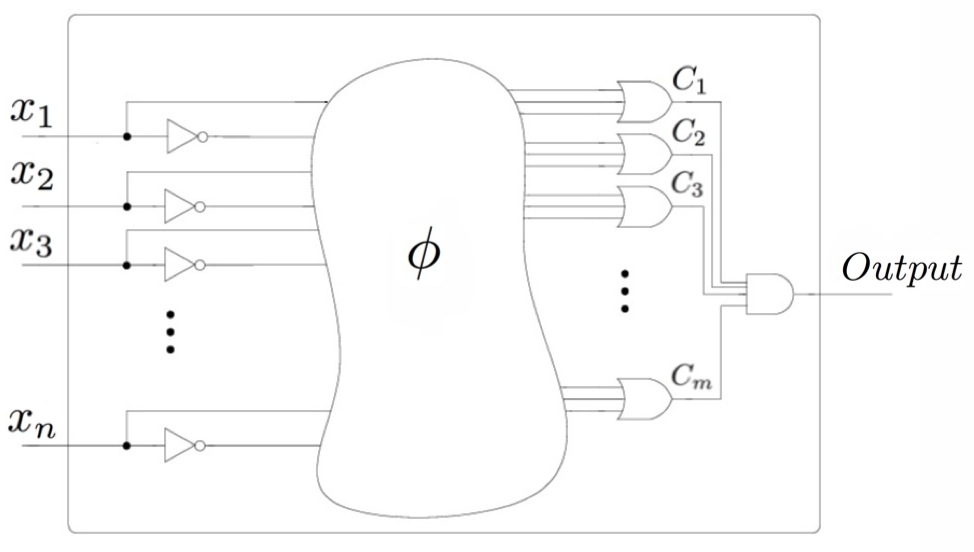
\includegraphics[width=0.9\textwidth]{figures/circuitLabeled.jpg}

\caption{A circuit describing {\sc Satisfiability}.}
\label{blackBoxSat}
\end{center}
\end{figure}
	
\FloatBarrier

%	<Paragraph> Provide complexity of {\sc Satisfiability}
The realization of {\sc Satisfiability} as a circuit shows two insights of the problem.  {\sc Satisfiability} can be implemented with logic components proportional to the problem size, and the worst case verification consists of enumerating all possible switch configurations.  {\sc Satisfiability} as a language demonstrates that it is equivalent to all other \textsf{NP-complete} languages.

Cook and Levin independently introduced the canonical instance of a \textsf{NP-complete} language {\sc Satisfiability}\cite{Cook:1971:CTP:800157.805047, levin1973}.  A \textsf{NP-complete} language is one that is in \textsf{NP} and \textsf{NP-hard}.  A \textsf{NP-hard} language is at least as hard as any problem in \textsf{NP}.

%	<Paragraph> Motivate practical input and classifying metrics 

The next section considers standards adopted for {\sc Satisfiability}.  This allows practitioners to apply {\sc Satisfiability} in various settings.
	
\section{Evaluating {\sc Satisfiability}}

%	<Paragraph> Overview of evaluation
	
	In this section, we describe two standards for encoding the {\sc Satisfiability} problem that we adopt for the implementation.  This includes the input and output standards for the {\sc Satisfiability} Competition \cite{dimacsFormat, satcompetition}.  
	
	Next, we introduce problem instance classification for {\sc Satisfiability}.  Classification of {\sc Satisfiability} problem instances include randomly generated, combinatorial, and industrial \cite{satcompetition}.  The experimental setup in Chapter 6 considers generation of random $k$-{\sc Sat} input.

	\subsection{Input and output}
	
%		<Paragraph> {\sc Satisfiability} standards [provide] common interface
	
%  Conforming to standards allows datasets and common interfaces to be shared.  
 Each year a competition showcases techniques for evaluating {\sc Satisfiability} \cite{satcompetition}.  We conform to the standards of the {\sc Sat} Competition \url{http://www.satcompetition.org/}.  {\sc Sat} solvers demonstrate state-of-the-art techniques for solving three main tracks of {\sc Satisfiability} instances.  The tracks exhibit applications for {\sc Satisfiability}, including: industrial applications, hard combinatorial, and random problem instances.
 
 The input and output standards for {\sc Satisfiability} allow common benchmarks for {\sc Sat} solvers.
	
		\subsubsection{Input}
		
%			<Paragraph> DIMACS CNF [provides] standard benchmark instances
DIMACS CNF provides a standard input for {\sc Satisfiability} \cite{dimacsFormat}.  The format permits sharing of existing {\sc Satisfiability} benchmarks by encoding {\sc Satisfiability} in conjunctive normal form (CNF).  The format is user readable with a natural encoding for {\sc Satisfiability}.  We provide an example of this encoding in Section \ref{inputSection}.
		
		\subsubsection{Output}
		
%			<Paragraph> Sat Competition output [provides] standard output

{\sc Sat} Competition output consists of the status for a DIMACS CNF input instance \cite{satcompetition}.  This includes the known state, either \texttt{SATISFIABLE}, \texttt{UNSATISFIABLE}, or \texttt{UNKNOWN}.  When a witnessing satisfying assignment occurs, the assignment gets provided as a list of integers with the \texttt{SATISFIABLE} state.  We provide an example along with a custom interface in Section \ref{outputSection}.
	
	\subsection{Metrics for classifying {\sc Satisfiability}}

%		<Paragraph> Describe metrics
{\sc Sat} phase transition and {\sc Sat} backbones are two classifying metrics for {\sc Satisfiability}.  These metrics may be used to classify {\sc Satisfiability} expressions.  We will use these metrics in the next section for defining a collection of random $k$-{\sc Sat} instances.
		
%		<Paragraph> {\sc Sat} phase transition

\begin{definition}
CNF\\
Conjunctive Normal Form consists of the intersection of sets of disjunctive literals. 
\end{definition}

\begin{definition}
$k$-CNF\\
Consists of a CNF expression with each disjunctive clause containing $k$ literals.
\end{definition}

\begin{definition}
$k$-{\sc Sat}\\
Problem variant of {\sc Satisfiability} where each clause consists of $k$ Boolean literals.  $k$-CNF formula provide an equivalent representation.
\end{definition}

\begin{definition}
{\sc Sat} phase transition\\
The {\sc Sat} phase transition is a region where both satisfiable and unsatisfiable instances are likely.  The ratio of clauses to variables $\alpha = m/n$ provides a characterization for where phase transitions may occur in the space of all $k$-CNF formula \cite{Doherty08thehandbook,Gent94thesat}.
\end{definition}
		
%		<Paragraph> {\sc Sat} backbones
\begin{definition}
{\sc Sat} backbones\\
{\sc Sat} backbones are the variable assignments present in all of the satisfying assignments to a {\sc Satisfiability} expression \cite{Zhang2001}.  This is a set of variables that occur in all satisfiable witnesses for an input expression.  

\end{definition}



	\subsection{{\sc Satisfiability} instances}
		
%		<Paragraph> Various methods for [constructing] {\sc Satisfiability} instances
There are several methods for constructing {\sc Satisfiability} instances.  We consider techniques for constructing instances based on random assignment, combinatorial, and real applications from industry.  The instance type demonstrate properties of {\sc Satisfiability} and provide heuristics for certain input.
	
%		<Paragraph> {\sc Satisfiability} instance [generated] from random assignment
A random $k$-{\sc Sat} expression consists of $m$ clauses with $k$ literals per-clause from  $n$ variables \cite{wilsonKsat}. Variable assignments get distributed with probability 
\[
Prob\left(\frac{1}{n}\right).
\]
\noindent The positive or negative variable polarity get assigned with a probability 
\[
Prob\left(\frac{1}{2}\right).
\]

%Random $k$-{\sc Sat} are generated with \texttt{ksat.c} \cite{wilsonKsat}.  A hash of the clause representation ensures that all clauses are independent \cite{wilsonKsat}.

%During generation of these formulas a hash is implemented to ensure that the random assignments ensure independent clauses and non-redundant variable assignments.  
		
%		<Paragraph> {\sc Satisfiability} instance [constructed] as hard assignment

Combinatorial instances provide difficult benchmark cases.  These instances can be converted from other \textsf{NP-complete} problems.  This category also includes games and graph theoretic problems represented as {\sc Satisfiability}. 
		
		
%		<Paragraph> {\sc Satisfiability} instance [applied] from real world problems

Industrial processes apply {\sc Satisfiability} in many real world problems.  This includes circuit layout, planning, logistics, circuit fault testing and many other industrial \textsf{NP-complete} problems.  Applications for industrial {\sc Sat} will often apply heuristics, and approximation techniques to relax the problem.  This allows approximate solutions to be computed in an efficient amount of time.
		